% !TEX root = ../main.tex

\chapter{Experiments}
\label{ch:experiments}

\section{Research Questions}
To analyze and compare the different models and their architectures, I formulated the following research questions:
\begin{enumerate}
  \item How do function approximators other than neural networks compare with the latter?
  \item Why did the models without bias generally perform better than the ones with bias?
  \begin{enumerate}
    \item Does increasing the number of weights worsen the performance of the model?
    \item Does a neural network with more than two hidden layers yield worse scores?
    \item Does the neural network's performance suffer from an increase in the number of neurons?
    \item Does the difficulty of the environment affect the observed effect of the bias?
  \end{enumerate}
\end{enumerate}

\section{Experiments}
To investigate and answer the formulated research questions, I conducted the following experiments:
\begin{enumerate}
  \item I selected a few promising models to analyze. They are described in Section~\ref{ssec:models}. Similar to \citet{oller_analyzing_2020}, I used RWG to draw the weights of the models and tested the performance on a Classic Control environment from OpenAI Gym.
  \item With the same settings for the experiments as in Section~\ref{ssec:benchmarks}, I varied the number of (a) weights, (b) hidden layers, and (c) neurons for a neural network and compared the results. In addition, I also increased the number of weights for the polynomial model.
  \item For this experiment, I used the same network architectures and procedure as explained in Section~\ref{ssec:benchmarks}. But this time, I chose environments with a higher difficulty level.
\end{enumerate}

\subsection{Experiment 1}
In the first experiment, analogous to \citet{oller_analyzing_2020}, there is no learning involved. For their paper, they were interested in the complexity of the environment, whereas I aim to find out more about the nature of the models. I selected a few candidates for the models, which are described in Section~\ref{ssec:models} and used them for a series of experiments. I used the same procedure for all models, which allows me to compare them with one another. For the experiments, first, I initialized the environment. I used the \verb|CartPole| and \verb|Acrobot| environment for these experiments. These environments are fairly easy to solve, as explained in Section~\ref{ssec:benchmarks}. Therefore, we expect some controllers to solve the task even without any training. Second, I initialized the respective model. Then, I drew the model weights from the standard normal distribution $\mathcal{N}(0,1)$. Each of these instances of the model represents a sample. In total, I used $10'000$ samples ($N_{samples}$). Finally, I ran 20 episodes ($N_{episodes}$) with each sample for an environment and stored the respective score as an entry of the score tensor $S$. Algorithm~\ref{alg:model-evaluation} shows an overview of the described procedure.
\begin{algorithm}
\caption{First experiment with RWG}
\begin{algorithmic}[1]
\State Initialize environment
\State Initialize model
\State Create array $S$ of size $N_{samples} \times N_{episodes}$
\For{$n = 1,2,...,N_{samples}$}
    \State Sample model weights randomly from $\mathcal{N}(0,1)$
    \For{$e=1,2,...,N_{episodes}$}
      \State Reset the environment
      \State Run episode with model
      \State Store accured episode reward in $S_{n,e}$
    \EndFor
\EndFor
\end{algorithmic}
\label{alg:model-evaluation}
\end{algorithm}

\subsection{Experiment 2}
For the second experiment, I used the same procedure as described in Section~\ref{ssec:benchmarks}. I used neural networks for all experiments. Additionally, I used the polynomial model for the experiment concerning the weights of the model.
\begin{enumerate}
  \item I used the same number of hidden layers and neurons for the neural networks as before: a network without hidden layers, a network with one hidden layer with four hidden units, and a network with two hidden layers and four hidden units for each layer. I only changed the number of weights for each network. In addition, I used the model $P_1$ described in Section~\ref{ssec:models}.

  First, I doubled the number of weights for all models. Then, I tripled the number of weights for all models. To achieve this, I constructed one weight $\mathbf{w_i}$ out of two, respectively, three weights by addition:
  \begin{align*}
    &\text{Double number of weights: } &\mathbf{w_i} &= \mathbf{w_{i1}} + \mathbf{w_{i2}} \\
    &\text{Triple number of weights: } &\mathbf{w_{i}} &= \mathbf{w_{i1}} + \mathbf{w_{i2}} + \mathbf{w_{i3}}
  \end{align*}
  \item In this experiment, I tested the models with different numbers of hidden layers. Each layer still has the same number of hidden neurons as before. Thus, the networks have four hidden units for each layer. I used a network with four hidden layers, one with six, and one with eight.
  \item For this experiment, I varied the number of hidden neurons for a network. I used a network with two hidden layers. For the number of hidden neurons, I chose 5, 8, and 10.
\end{enumerate}
\todo[inline]{Maybe add table with used architecture to make it more comprehensible \\ Add more neurons?}

\subsection{Experiment 3}
For this experiment, I used the same network architectures as \citet{oller_analyzing_2020}: a neural network wihtout any hidden layers, one with one hidden layer and four hidden units, and one with two hidden layers and four hidden units for each layer. The procedure of the experiment is also analogous to the one conducted in the paper. The only thing that I vary is the choice of the environment. The environments represent a gradually increase in complexity. \\
\todo[inline]{Try with RWG. If not possible to get any results, use CMA-ES. \\ Environments: Original Pendulum, Inverted Double Pendulum, Swing Up Double Pendulum?}

\subsection{OpenAI Gym Environments}
\begin{itemize}
  \item CartPole
  \item Acrobot
  \item Pendulum
\end{itemize}

\todo[inline]{Explain used environments, maybe put into Introduction section}

\subsection{Models}
\label{ssec:models}
For the polynomial model, I used two architectures $P_1$ and $P_2$. The first model $P_1$ consists of one polynomial for each possible action in a discrete action space. The input of the model is the observation from the environment. The dimension of the weight vectors is according to the dimension of the input vector. For the environment \verb|CartPole| with the discrete action space $\{0, 1\}$ and observation $\mathbf{x} = [x_0, x_1, x_2, x_3]^T$, this means that $P_1$ consists of two polynomials:
\begin{align*}
  &p_0(\mathbf{x}) = \Sigma_{i=0}^{n} \mathbf{w_i}^T (x_k^i)_{k \in I} \in \mathbb{R}, &\mathbf{w_0}, ..., \mathbf{w_3}, \mathbf{x} \in \mathbb{R}^4, \ \ I = \{0, 1, 2, 3\} \\
  &p_1(\mathbf{x}) = \Sigma_{i=0}^{n} \mathbf{\hat{w}_i}^T (x_k^i)_{k \in I} \in \mathbb{R}, &\mathbf{\hat{w}_0}, ..., \mathbf{\hat{w}_3}, \mathbf{x} \in \mathbb{R}^4, \ \ I = \{0, 1, 2, 3\}
\end{align*}
In the formulas, $n$ denotes the degree of the polynomial. In my experiments, I tested polynomials of degrees 1, 2, and 3. The output of the polynomials has no reasonable upper and lower limit, as illustrated in Figure~\ref{fig:bounds}. That makes it harder to interpret the results reasonably.
\begin{figure}[ht]
\centering
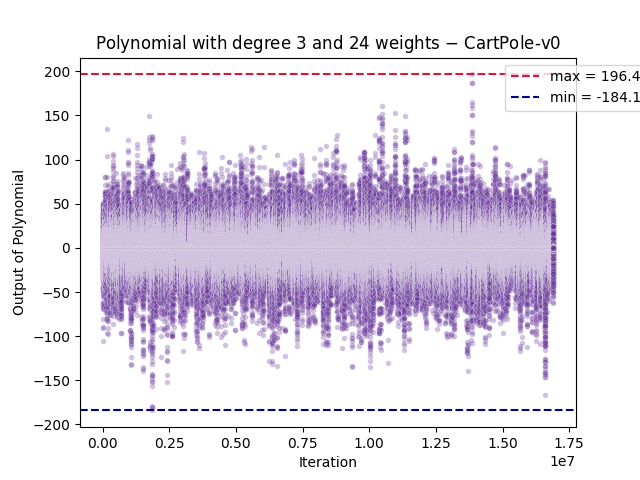
\includegraphics[width=0.6\textwidth]{PolynomialNN_degree_3_bounds}
\caption[Upper and lower bound]{
  \textbf{Upper and lower bound.}
  The figure shows each output of the polynomial functions described above. As we can see, the functions are not well bound, and there are quite a few outliers. That makes it hard to interpret the output sensibly.
}
\label{fig:bounds}
\end{figure}
So, I scaled the outputs with a sigmoid function. A sigmoid function is a mathematical function that maps an arbitrary input space into an output space with a small range, for example, 0 and 1. The function has a characteristic S-shaped curve. We can interpret the output space of the sigmoid function as a probability. In this case, we search for the probability that a specific action is the reasonable one given an observation $\mathbf{x}$. Thus, for our example with the \verb|CartPole| environment, we can interpret $sig(p_0)$ as the probability that action 0 is the correct one and $sig(p_1)$ as the probability that action 1 is the correct one. Putting this thought into a formula for $P_1$ and the \verb|CartPole| environment, we get:
\[
  P_1(\mathbf{x}) =
  \begin{cases}1~&{\text{ if }}~sig(p_1(\mathbf{x})) > sig(p_0(\mathbf{x}))~,\\0~&~\text{otherwise}~.\end{cases}
\]
For the sigmoid function, I used the logistic sigmoid function. The formula and a plot of the function in 2D are shown in Figure~\ref{fig:sigmoid}.
\begin{figure}[ht]
\centering
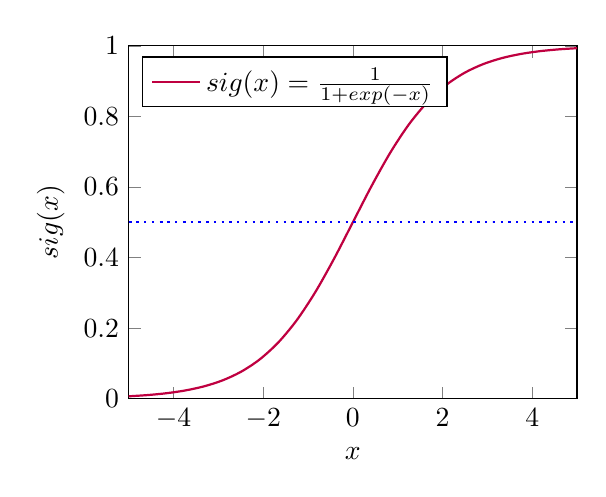
\begin{tikzpicture}
\begin{axis}[
      xmin = -5, xmax = 5,
      ymin = 0, ymax = 1,
      legend cell align = {left},
      legend pos = north west,
      width = 0.6\textwidth,
      height = 0.5\textwidth,
      xlabel = \(x\),
      ylabel = {\(sig(x)\)}
    ]
    \addplot[
        smooth,
        thick,
        purple
    ] {1 / (1 + exp(-x))};
    \addlegendentry{
    $sig(x) = \frac{1}{1 + exp(-x)}$
    }
    \addplot[
        smooth,
        thick,
        blue,
        dotted
    ] {0.5};
\end{axis}
\end{tikzpicture}
\caption[Sigmoid function]{
  \textbf{Sigmoid function.}
  The figure shows a plot of the logistic sigmoid function. The function maps an arbitrary input space into the range between 0 and 1. The output of the function can be interpreted as a probability. It is useful to scale data into a meaningful value.
}
\label{fig:sigmoid}
\end{figure}

The second model $P_2$ is constructed similarly to $P_1$, but it only consists of one polynomial instead of one for each possible action. For the \verb|CartPole| environment, this means $P_2$ consists of:
\[
  p(\mathbf{x}) = \Sigma_{i=0}^{n} \mathbf{w_i}^T (x_k^i)_{k \in I} \in \mathbb{R}, \ \ \ \ \ \ \ \ \ \ \mathbf{w_i} \in \mathbb{R}^4, \ \ I = \{0, 1, 2, 3\}
\]
Analogous to $P_1$, I tested the polynomial $p(\mathbf{x})$ with degrees 1, 2, and 3. So, $n \in \{1, 2, 3\}$. In addition, I again used the logistic sigmoid function to scale the output of the polynomial. However, the output of $P_2$ is determined by a fixed threshold instead of comparing multiple polynomials. Putting this into a formula for the \verb|CartPole| environment, we get:
\[
  P_2(\mathbf{x}) =
  \begin{cases}1~&{\text{ if }}~sig(p(\mathbf{x}))>0.5~,\\0~&~\text{otherwise}~.\end{cases}
\]


\section{Results}
\subsection{Experiment 1}
Figure~\ref{fig:experiment_1_polynomial} shows the results of the first experiment for the two architectures of the polynomial model $P_1$ and $P_2$. I visualized the results of each model with bias connection in row (a) and without bias connection in row (b). The structure of the plots is identical for better comparison. The samples are ranked according to their mean score and aligned on the $x-$axis according to their rank. The scatter plots show all scores of the samples, whereas the lineplot illustrates the mean of each sample over all episodes.
Subfigure~\ref{fig:results_p1} shows the results of the polynomial model $P_1$ and Subfigure~\ref{fig:results_p2} shows the results of the polynomial model $P_2$.
\begin{figure}[!ht]
\begin{subfigure}{\textwidth}
\begin{figrow}
\item \label{row:P1_with_bias} \raisebox{-0.5\height}{
\includegraphics[width=.3\linewidth]{experiment_1/with_bias/PolynomialNN_degree_1_scatter_score.png}
\includegraphics[width=.3\linewidth]{experiment_1/with_bias/PolynomialNN_degree_2_scatter_score.png}
\includegraphics[width=.3\linewidth]{experiment_1/with_bias/PolynomialNN_degree_3_scatter_score.png}}
\item \label{row:P1_without_bias}  \raisebox{-0.5\height}{
\includegraphics[width=.3\linewidth]{experiment_1/without_bias/PolynomialNN_degree_1_scatter_score.png}
\includegraphics[width=.3\linewidth]{experiment_1/without_bias/PolynomialNN_degree_2_scatter_score.png}
\includegraphics[width=.3\linewidth]{experiment_1/without_bias/PolynomialNN_degree_3_scatter_score.png}}
\end{figrow}
\vspace*{-5mm}
\caption{Results of $P_1$ with bias (a) and without bias (b)}
\label{fig:results_p1}
\end{subfigure}
\begin{subfigure}{\textwidth}
\begin{figrow}
\item \label{row:P2_with_bias} \raisebox{-0.5\height}{
\includegraphics[width=.3\linewidth]{experiment_1/with_bias/Polynomial_degree_1_scatter_score.png}
\includegraphics[width=.3\linewidth]{experiment_1/with_bias/Polynomial_degree_2_scatter_score.png}
\includegraphics[width=.3\linewidth]{experiment_1/with_bias/Polynomial_degree_3_scatter_score.png}}
\item \label{row:P2_without_bias}  \raisebox{-0.5\height}{
\includegraphics[width=.3\linewidth]{experiment_1/without_bias/Polynomial_degree_1_scatter_score.png}
\includegraphics[width=.3\linewidth]{experiment_1/without_bias/Polynomial_degree_2_scatter_score.png}
\includegraphics[width=.3\linewidth]{experiment_1/without_bias/Polynomial_degree_3_scatter_score.png}}
\end{figrow}
\vspace*{-5mm}
\caption{Results of $P_2$ with bias (a) and without bias (b)}
\label{fig:results_p2}
\end{subfigure}
\caption[Results of experiment 1: polynomial models]{
  \textbf{Results of experiment 1: polynomial models.}
   The figures show the results of the first experiment with the two polynomial models. On the $x-$axis, we have the rank of each sample. On the $y-$axis, we have the scores of all samples and the mean as a lineplot. Each subplot shows the performance of the model with bias in row (a) and without bias in row (b). As we can see, both models perform equally good or bad. However, there is a huge difference in performance whether we are working with or without bias. In addition, we can see a difference in the slope of the mean values between polynomials with degree 1 and one with a higher degree.
}
\label{fig:experiment_1_polynomial}
\end{figure}
As we can see in the images, the plots of the two models almost look identical. Both models performed equally good or bad despite their different architecture and the different number of weights. Because of this similarity, I will not go into each model independently but instead discuss further results for both of them.

Looking at the linear model without bias, we can see a striking resemblance to the performance of the neural network previously shown in Section~\ref{ssec:benchmarks}. Looking further at the linear model, we can see that the curve of the mean score stays low until around $5'000$ but then goes up relatively steeply. That means that the linear model fails around 50\% miserably. However, after that, we have a high probability to achieve a good score or even solve the task entirely during multiple episodes. There are also quite a few samples that could solve the task each time, indicated by the short straight black line at the top of the plot. Looking at the polynomials with degree 2, we can see that the scores increase already at around $2'000$, but the slope is less steep than for the linear model. In addition, there are fewer samples that could solve the task for each episode than there are for the linear model. Furthermore, the variance is higher for the polynomials with a higher degree compared to the linear model. If we look at the results of the polynomials with degree three, we can see that there is only a small boost compared to the polynomials of degree 2. The scores are overall slightly higher, but the slope is very similar to before. There is only a little difference between the two models even though the weights are doubled for $P_1$ and a half more for $P_2$. The large difference lies between the polynomials with degree 1 and polynomials with degree 2, respectively, degree 3. It seems that the complexity of the model depends more on the architecture of the model than on the number of weights.

In conclusion, with the linear model, we have a $50 \%$ chance of failing but the probability of actually solving the task for all episodes is higher than for the polynomials with a higher degree. That means that with the linear model, we have a larger fraction of samples that can solve the environment independent of the initialization conditions. At first glance, we could assume that this is an important aspect for such a model and choose the polynomial with degree 1 over one with a higher degree. However, we should remind ourselves that these experiments are rather unusual for an application since there is no learning involved and the number of samples is huge. In a common application, we would use some kind of training and want the model to sequentially improve its performance. Considering this aspect, when using a learning algorithm, we would not prefer the polynomials with degree 1 as we might get stuck in a fitness plateau when the algorithm has no method of dealing with this behavior.

Another observation we can make from Figure~\ref{fig:experiment_1_polynomial} is that the bias influences the performance of the model significantly. We already saw this behavior with the neural network in Section~\ref{ssec:benchmarks}. Thus, the influence of the bias is not specific to neural networks but seems to be more of a general factor.

\todo[inline]{Change title of plots: , instead of with, $P_1 / P_2$ instead of Polynomial \\ Explain fitness plateau further}

\subsection{Experiment 2}
Figure~\ref{fig:experiment_2_default} shows the results of the three neural network architectures that were mentioned in Section~\ref{ssec:benchmarks}. Row (a) shows the results with bias connection, whereas row (b) shows the results with dropping bias connection. These plots show the results with the default network architectures.

\begin{figure}[!ht]
\begin{figrow}
\item \label{row:NN_with_bias_default} \raisebox{-0.5\height}{
\includegraphics[width=.3\linewidth]{experiment_2/default/with_bias/HL_0_HU_0_scatter_score.png}
\includegraphics[width=.3\linewidth]{experiment_2/default/with_bias/HL_1_HU_4_scatter_score.png}
\includegraphics[width=.3\linewidth]{experiment_2/default/with_bias/HL_2_HU_4_scatter_score.png}}
\item \label{row:NN_without_default}  \raisebox{-0.5\height}{
\includegraphics[width=.3\linewidth]{experiment_2/default/without_bias/HL_0_HU_0_scatter_score.png}
\includegraphics[width=.3\linewidth]{experiment_2/default/without_bias/HL_1_HU_4_scatter_score.png}
\includegraphics[width=.3\linewidth]{experiment_2/default/without_bias/HL_2_HU_4_scatter_score.png}}
\end{figrow}
\caption[Plots of neural networks with default configurations]{
  \textbf{Plots of neural networks with default configurations.}
   The plots show the results of the default configuration of a neural network taken from the paper. Row (a) shows the results with bias connections, whereas row (b) shows the results without bias connections.
}
\label{fig:experiment_2_default}
\end{figure}

Figure~\ref{fig:experiment_2_weights} shows the results of tripling the number of weights for each network architecture. Row (a) shows the results using bias, row (b) shows the results without bias. I did not include the results where I doubled the weights since there was very little difference visible in the plots. Comparing the plots from Figure~\ref{fig:experiment_2_weights} with the ones from Figure~\ref{fig:experiment_2_default}, we can barely see any difference. The slope of the mean values looks the same. The data points do not show different behavior. That applies to both rows (a) and rows (b). Thus, we can conclude that increasing the number of weights does not impact the achieved score of the model significantly. In addition, I conducted the same experiment with the polynomial models $P_1$ and $P_2$. We can make the same observation with these models.
\begin{figure}[!ht]
\begin{figrow}
\item \label{row:NN_with_bias_wfactor_3} \raisebox{-0.5\height}{
\includegraphics[width=.3\linewidth]{experiment_2/weights/weight_factor_3/with_bias/HL_0_HU_0_scatter_score.png}
\includegraphics[width=.3\linewidth]{experiment_2/weights/weight_factor_3/with_bias/HL_1_HU_4_scatter_score.png}
\includegraphics[width=.3\linewidth]{experiment_2/weights/weight_factor_3/with_bias/HL_2_HU_4_scatter_score.png}}
\item \label{row:NN_without_bias_wfactor_3}  \raisebox{-0.5\height}{
\includegraphics[width=.3\linewidth]{experiment_2/weights/weight_factor_3/without_bias/HL_0_HU_0_scatter_score.png}
\includegraphics[width=.3\linewidth]{experiment_2/weights/weight_factor_3/without_bias/HL_1_HU_4_scatter_score.png}
\includegraphics[width=.3\linewidth]{experiment_2/weights/weight_factor_3/without_bias/HL_2_HU_4_scatter_score.png}}
\end{figrow}
\vspace*{-5mm}
\caption[Results of experiment 2: weights]{
  \textbf{Results of experiment 2: weights.}
   The figure shows the results of tripling the number of weights for the three neural network architectures. Row (a) shows the results with bias connections, row (b) shows the results without bias connections. Despite the increased number of weights, there is no visible difference in the plots compared to the ones shown in Figure~\ref{fig:experiment_2_default}.
}
\label{fig:experiment_2_weights}
\end{figure}


Figure~\ref{fig:experiment_2_layers} shows the results of altering the number of layers in a network. For the networks with bias connections, the performance gets significantly worse with an increased number of layers. The networks without bias connections seem to be more robust. Still, the steepness of the slope of the line plots decreases with an increased number of layers.
\begin{figure}[!ht]
\begin{figrow}
\item \label{row:NN_with_bias_layers} \raisebox{-0.5\height}{
\includegraphics[width=.3\linewidth]{experiment_2/layers/with_bias/HL_4_scatter_score.png}
\includegraphics[width=.3\linewidth]{experiment_2/layers/with_bias/HL_6_scatter_score.png}
\includegraphics[width=.3\linewidth]{experiment_2/layers/with_bias/HL_8_scatter_score.png}}
\item \label{row:NN_without_layers}  \raisebox{-0.5\height}{
\includegraphics[width=.3\linewidth]{experiment_2/layers/without_bias/HL_4_scatter_score.png}
\includegraphics[width=.3\linewidth]{experiment_2/layers/without_bias/HL_6_scatter_score.png}
\includegraphics[width=.3\linewidth]{experiment_2/layers/without_bias/HL_8_scatter_score.png}}
\end{figrow}
\caption[Results of experiment 2: layers]{
  \textbf{Results of experiment 2: layers.}
   The plots show the result of increasing the number of hidden layers gradually. Again, row (a) represents the networks with bias connections, row (b) the ones without bias connections. As we can see, the results in row (a) get worse with an increase in the number of layers. Row (b) is less extreme but there is also a loss of steepness with an increasing number of hidden layers.
}
\label{fig:experiment_2_layers}
\end{figure}

Figure~\ref{fig:experiment_2_neurons} shows the results of increasing the number of neurons in each hidden layer for a network with two hidden layers. Comparing the plots with the ones in Figure~\ref{fig:experiment_2_default}, we can see a slight improvement in the plots without bias connections in rows (a). In addition, the data points seem to be more spread out, indicating a higher variance. The results of the networks without using bias connections do not show much difference. The slope is a little less steep with increased neurons.
\begin{figure}[!ht]
\begin{figrow}
\item \label{row:NN_with_bias_neurons} \raisebox{-0.5\height}{
\includegraphics[width=.3\linewidth]{experiment_2/neurons/with_bias/HL_2_HU_5_scatter_score.png}
\includegraphics[width=.3\linewidth]{experiment_2/neurons/with_bias/HL_2_HU_8_scatter_score.png}
\includegraphics[width=.3\linewidth]{experiment_2/neurons/with_bias/HL_2_HU_10_scatter_score.png}}
\item \label{row:NN_without_neurons}  \raisebox{-0.5\height}{
\includegraphics[width=.3\linewidth]{experiment_2/neurons/without_bias/HL_2_HU_5_scatter_score.png}
\includegraphics[width=.3\linewidth]{experiment_2/neurons/without_bias/HL_2_HU_8_scatter_score.png}
\includegraphics[width=.3\linewidth]{experiment_2/neurons/without_bias/HL_2_HU_10_scatter_score.png}}
\end{figrow}
\caption[Results of experiment 2: neurons]{
  \textbf{Results of experiment 2: neurons.}
  The plots show the result of increasing the number of neurons for each layer in a network with two hidden layers. The plots in row (a) represent the networks with bias connections, the ones in row (b) represent the networks without bias connections. We can see a slight improvement in row (a).
}
\label{fig:experiment_2_neurons}
\end{figure}

\todo[inline]{Improve interpretation, mention that these are feed forward networks (maybe experiments descr)}
